\chapter{Text classification}
Information extraction from the text can be stated as a text classification task.
Given a text, we want to assign a class it belongs to.
The class can be anything, from the text's category to the text's sentiment or the author's age.
Depending on the number of classes, we can distinguish between \textbf{binary} (2) and \textbf{multiclass} (2+) classification.
We might want to classify the text by multiple labels; we thus also distinguish between \textbf{single-label}
and \textbf{multi-label} classification.

Therefore, we can rephrase our research question as a \textbf{single-label multiclass text classification of Czech News articles}.
To avoid ambiguity, we will refer to a single news article text as a \textbf{document} going forward.

\section{Evaluation Metrics}
\label{sec:metrics}
To assess performance, we need to define some metrics.
We start by defining metrics for binary classification and then extend them to multiclass classification.

In Binary classification, we have two classes; positive and negative. Thus we can have four possible outcomes:
\begin{enumerate}
    \item \ac{tp} - prediction positive, label positive
    \item \ac{tn} - prediction negative, label negative
    \item \ac{fn} - prediction negative, label positive
    \item \ac{fp} - prediction positive, label negative
\end{enumerate}

The most basic metric is accuracy, which is defined as
\begin{equation*}
    \label{eq:accuracy}
    \operatorname{Accuracy} = \frac{\mathrm{TP} + \mathrm{TN}}{\mathrm{TP} + \mathrm{TN} + \mathrm{FP} + \mathrm{FN}}
\end{equation*}
However, accuracy often fails to capture the whole picture.
Let's consider a dataset of 1000 people, where 990 are healthy and 10 are sick.
Such a dataset is called \textbf{imbalanced}, as the number of classes is distributed unequally.
We will consider sick people to be positive class and healthy people to be negative class.
On this dataset, we could achieve 99\% accuracy by always predicting that the person is healthy.
Such a model would be useless in practice, as it could not detect sick people.

\subsection{Precision and Recall}
Precision and recall deal with the issue of imbalanced datasets.
They are defined as
\begin{equation*}
    \label{eq:precision}
    \operatorname{Precision} = \frac{\mathrm{TP}}{\mathrm{TP} + \mathrm{FP}}
\end{equation*}
\begin{equation*}
    \label{eq:recall}
    \operatorname{Recall} = \frac{\mathrm{TP}}{\mathrm{TP} + \mathrm{FN}}
\end{equation*}
Considering the same model, we will score 0\% recall and undefined precision.
If we were to increase the recall by always predicting sick, we would achieve 100\% recall and 1\% precision.
A good model should thus have both high precision and recall.

\subsection{$F_{\beta}$ Score}
The $F_{\beta}$ score answers our requirements.
It combines precision and recall into one metric and is defined as
\begin{equation*}
    \label{eq:f1}
    F_{\beta} = (1 + \beta^2) \cdot \frac{\operatorname{Precision} \cdot \operatorname{Recall}}{\beta^2 \cdot \operatorname{Precision} + \operatorname{Recall}}
\end{equation*}
We can control the importance of precision and recall by changing the $\beta$ parameter.

\subsection{Micro and Macro Averaging}
We can use micro and macro averaging to extend the binary metrics to a multiclass case.
In the case of micro averaging, we consider $\mathrm{TP}, \mathrm{TN}, \mathrm{FP}$ and $\mathrm{FN}$ as the sum of respective values for each class.
We then calculate the metrics as before.
In the case of macro averaging, we calculate the metrics for each class and then average them.
This results in treating each class equally irregardless of the number of samples in each class.

\subsection{Interannotator Agreement and Cohen's Kappa}
\label{sec:interannotator}
One can use the \textbf{Cohen's kappa} metric to assess agreement between annotators.
Assume we have two annotators annotating a dataset of $n$ samples with $k$ classes.
Denote class annotated by annotator $i$ to sample $j$ as $c_{ij}$.
Denote a total number of samples annotated by annotator $i$ as class $c$ as $n_{ic}$.
We can then calculate Cohen's kappa as
\begin{equation*}
    \label{eq:kappa}
    \kappa = \frac{p_o - p_e}{1 - p_e}
\end{equation*}
where $p_o$ is the observed agreement and $p_e$ is the expected agreement.
The expected agreement is calculated as
\begin{equation*}
    \label{eq:pe}
    p_e = \sum_{i=1}^k \frac{n_{1i} n_{2i}}{n^2}
\end{equation*}
The observed agreement is calculated as
\begin{equation*}
    \label{eq:po}
    p_o = \frac{1}{n} \sum_{i=1}^n \frac{c_{1i} = c_{2i}}{n}
\end{equation*}
The interpretation of the metric is not well established, as
it is unclear how high the metric should be to be considered good.
\textcite[page 165]{landisMeasurementObserverAgreement1977} suggest the following interpretation:
\begin{itemize}
    \item $\kappa < 0$ - poor agreement
    \item $0 \leq \kappa < 0.2$ - slight agreement
    \item $0.2 \leq \kappa < 0.4$ - fair agreement
    \item $0.4 \leq \kappa < 0.6$ - moderate agreement
    \item $0.6 \leq \kappa < 0.8$ - substantial agreement
    \item $0.8 \leq \kappa < 1$ - almost perfect agreement
\end{itemize}

\section{Notation intermezzo}
\label{sec:notation}
From now on, we will use the following notation:
\begin{itemize}
    \item non-bold lowercase letters (e.g. $x$) will denote a scalar.
    \item bold lowercase letters (e.g. $\mathbf{x}$) will denote a vector.
    \item bold uppercase letters (e.g. $\mathbf{X}$) will denote a matrix.
    \item letters with hat (e.g. $\hat{x}$) will denote a predicted value.
    \item $|V|$ will denote size of set $V$.
\end{itemize}
All vectors are column vectors unless otherwise stated.

\section{Document Representation}
\label{sec:representation}
To train a model, we need to represent the document in a way the model can understand.
Let's consider a dataset $D$ of $N$ documents. We can use the following representations:

\subsection{\acl{bow}}
\label{sec:bow}
One way to represent the document is to encode each word based on the number of occurrences in the document.
Such is an idea of the \acf{bow}. To obtain a \ac{bow} representation, we do the following:
\begin{enumerate}
    \item Tokenize the dataset. This is a process of splitting the text into smaller units called tokens (usually words).
    \item Create a vocabulary $V$ of all the tokens in the dataset.
    \item Represent document $d$ as vector of weights $(C_{d}^1, C_{d}^2, \dots, C_{d}^{|V|})$, where $C_{d}^i$
          is the number of occurrences of token $i$ in document $d$.
\end{enumerate}
This representation allows us to store the dataset as a sparse $N \cdot |V|$ matrix.

\subsection{TF-IDF}
\label{sec:tfidf}
TF-IDF is an extension of the \ac{bow} representation, where we also consider the document's token frequency.
To represent the weight of token $t$ in document $d$, we use the following formula:
\begin{equation*}
    \label{eq:tfidf}
    \operatorname{TF-IDF}(t, d) = \operatorname{TF}(t, d) \cdot \operatorname{IDF}(t)
\end{equation*}
where TF and IDF are defined as
\begin{equation*}
    \label{eq:tf}
    \operatorname{TF}(t, d) = \frac{C_{d}^t}{\sum_{j \in V} C_{d}^{j}}
\end{equation*}
\begin{equation*}
    \label{eq:idf}
    \operatorname{IDF}(t) = \log \frac{|D|}{\sum_{d \in D} (C_{d}^t)}
\end{equation*}


\subsection{Subword Representations}
The problem with preceding representations is that they cannot capture unseen words and require
an extensive vocabulary. To solve this problem, we can use subword representations. Unlike the previous
representations, subword representations are not fixed-sized.

\subsubsection{\acl{bpe}}
\label{sec:bpe}
Popularized by \textcite{sennrichNeuralMachineTranslation2016b}, the \acf{bpe} algorithm is following:
\begin{enumerate}
    \item Split sentences into words by whitespace and punctuation.
    \item Split each word into separate characters and add the special end of the word token.
    \item Initializes the vocabulary with all the found characters and the end of the word token.
    \item Iteratively merge the most frequent pair of characters into a single character.
    \item Stop when the vocabulary size reaches the desired size.
\end{enumerate}
We then use the vocabulary to encode the document as a sequence of token ids.

\subsubsection{WordPiece}
\label{sec:wordpiece}
WordPiece is a modification of \ac{bpe} that uses a different merging
strategy and pre-tokenization. It was first introduced by~\textcite{schusterJapaneseKoreanVoice2012}
and improved by~\textcite{wuGoogleNeuralMachine2016}.
For pre-tokenization, it adds a special token at the beginning instead of the end of the word.
As for the merging strategy, we choose the pair that maximizes the likelihood of the training data when merged.

\subsubsection{\acl{spm}}
\label{sec:spm}
Introduced by~\textcite{kudoSentencePieceSimpleLanguage2018}, \acf{spm} is rather a modular tokenizer than an algorithm.
It unifies the preprocessing and tokenization steps and allows different sub-word algorithms to be used.
Among other things, it also addresses the problem of encoding multiple space characters, which is impossible in the above sub-word algorithms.
It does so by introducing a special token for the space character.


\subsubsection{\acl{bbpe}}
\label{sec:bbpe}
First described by~\textcite{Radford2019LanguageMA}, \acf{bbpe} is a modification of \ac{bpe}.
It doesn't split into words and characters but directly into bytes.
The authors noticed that the encoding was doing suboptimal merges as adding exclamation marks to the end of the words.
To solve this problem, merges can only happen between the same character categories.

\section{\acl{ml} Models}
\label{sec:models}
This section reviews the \ac{ml} models we will use in experiments.
Our intention is not to provide a comprehensive review of text classification approaches.
If the reader is interested in such a work, we recommend work by \textcite{kowsariTextClassificationAlgorithms2019}.
We will not review either \acp{cnn} or \acp{rnn}.
However, we will refer to them and expect the reader to know them.

\subsection{\acl{mlr}}
\label{sec:mlr}
\acf{mlr} is a simple linear model.
The \ac{mlr} with $k$ classes is represented by matrix of weights $\mathbf{W} \in R^{k, d} = (\mathbf{w_1}, \mathbf{w_2}, \dots \mathbf{w_n})^T$
and vector of biases $\mathbf{b} = (\beta_1, \beta_2, \dots \beta_k)$.

Given input $\mathbf{x} \in R^{d}$, with correct class $C_t$, the probability of model predicting class $C_i$ is given by
\begin{align*}
    %% Softmax
    \operatorname{softmax}(\mathbf{z})          & = \frac{e^{z_i}}{\sum_{j=1}^{k} e^{z_j}}     \\
    %% Probability
    P(C_i | \mathbf{x}; \mathbf{W}, \mathbf{b}) & = \sigma(\mathbf{W} \mathbf{x} + \mathbf{b})
\end{align*}
The optimized loss function is cross-entropy loss:
\begin{equation*}
    \mathcal{L}(\mathbf{x};\mathbf{W}, \mathbf{b}) = \log{P(C_t \mathbf{x}; \mathbf{W}, \mathbf{b})}
\end{equation*}

The model is simple, so it can't capture complex relationships between features.
However, it serves as a good baseline model, and unlike later models, it can be easily interpreted.

\subsection{Transformers}
\label{sec:transformers}
Transformers have been first proposed for machine translation by \textcite{vaswaniAttentionAllYou2017d}.
They have since become a \ac{sota} model for many \ac{nlp} tasks, including Text Classification.
The original paper suggested using encoder-decoder architecture due to the nature of the machine translation task.
However, for text classification, there is no need for the decoder. Thus, the architecture can be simplified to only the encoder.
In the following sections by \textbf{transformer}, we will refer to the encoder part of the architecture.

\subsubsection{Architecture}
%import pdf
\begin{figure}[ht]
    \centering
    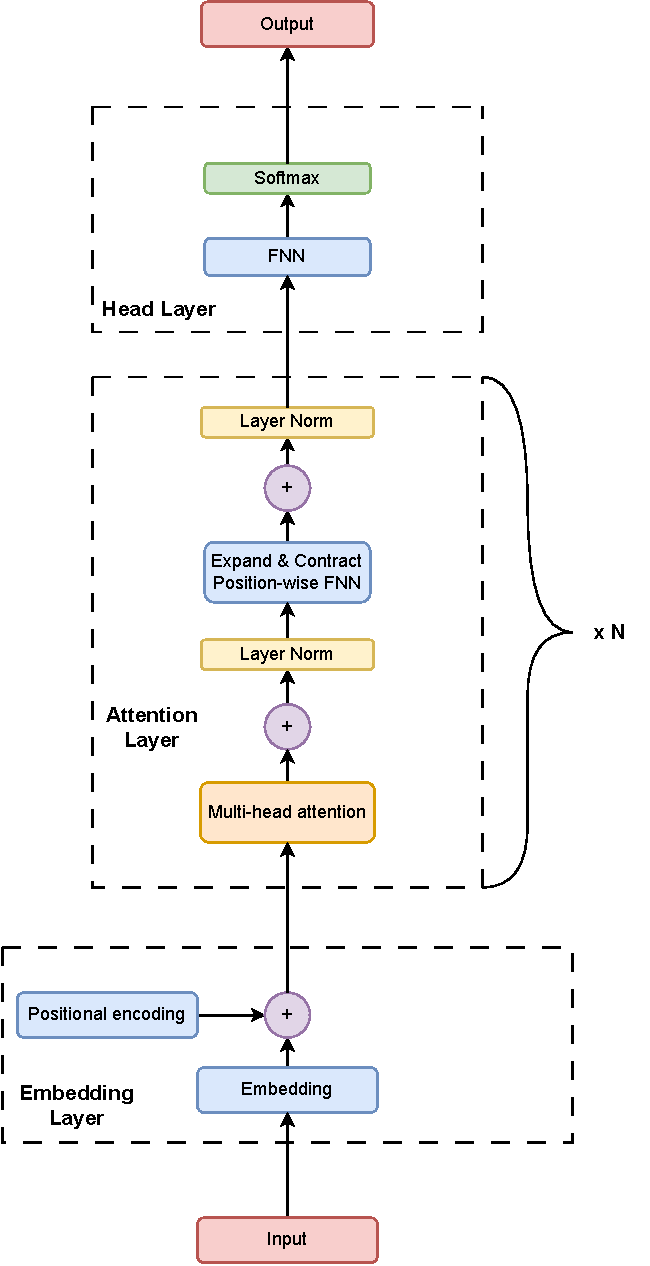
\includegraphics[width=0.7\linewidth]{img/transformer/trans_architecture.pdf}
    \caption{Transformer architecture without Dropout blocks for clarity.}
    \label{fig:transformer}
\end{figure}

The architecture of the transformer can be seen at \autoref{fig:transformer}.
The key components are
\begin{itemize}
    \item Embedding layer
    \item Multi-Head Attention Block
    \item Head layer
\end{itemize}
We will now describe each of them in detail.
\subsubsection{Embedding Layer}
The first layer of the transformer is an embedding layer, it takes the input text encoded as a vector $\mathbf{x} \in R^{n}$, with values in the range $[0, V)$, where $V$ is the vocabulary size.
The embedding layer embeds each vector element into vector space by employing a learnable matrix $\mathbf{E} \in R^{V, d}$, where $d$ is the arbitrary embedding dimension.
To encode the word's position in the sentence, we add a learnable positional embedding $\mathbf{P} \in R^{n, d}$.
Thus, the output of the embedding layer is given by
\begin{equation*}
    \mathbf{O} = \operatorname{OneHot}(\mathbf{x}) \cdot \mathbf{E} + \mathbf{P}
\end{equation*}
where $\operatorname{OneHot}(\mathbf{x})$ is a matrix of one-hot vectors, where each row corresponds to the one-hot vector of the corresponding element in $\mathbf{x}$.
This makes the model only accept fixed-length inputs.~\footnote{The original paper allowed for variable length inputs by employing a different strategy for positional encoding.}

\subsubsection{Self-attention}
Self-attention is a key mechanism of transformer architecture.
The Queries ($\mathbf{Q}$), Keys ($\mathbf{K}$), and Values ($\mathbf{V}$) matrices are computed from inputs as follows
\begin{align*}
    \mathbf{Q}                                             & = \mathbf{X} \mathbf{W_q}                  \\
    \mathbf{K}                                             & = \mathbf{X} \mathbf{W_k}                  \\
    \mathbf{V}                                             & = \mathbf{X} \mathbf{W_v}                  \\
    \text{where } \mathbf{W_q}, \mathbf{W_k}, \mathbf{W_v} & \in R^{d, d} \text{are trainable matrices}
\end{align*}
The output of the self-attention layer is then computed as follows~\footnote{The dimension hidden state of self-attention can be different from the embedding dimension. We use the same for simplicity.}
\begin{align*}
    \mathbf{O} & = \operatorname{softmax}\left(\frac{\mathbf{Q} \mathbf{K}^T}{\sqrt{d}}\right) \mathbf{V} \\
    \label{eq:attention}
\end{align*}
The intuition behind the self-attention is that by doing a scalar product between query and key vectors,
the model learns to focus on the most relevant parts of the input.
Such parts will then have the highest weight in the output in values multiplication.

\subsubsection{Multihead attention}
The multi-head attention is an extension of self-attention.
Instead of doing just one attention, we do multiple attentions in parallel, every attention with different Query, Key and Value matrices.
The outputs are then concatenated and passed through a linear layer.

\subsubsection{Head Layer}
Head Layer is task-dependent, as its task is to convert the transformer's output to the desired output.

\subsubsection{Benefits and Drawbacks}
\label{sec:benefits-and-drawbacks}
What transformers mostly improved were two things:
\begin{itemize}
    \item Capturing of long-range dependencies.
    \item Parallelization of the model. Unlike \acp{rnn}, we don't process a single input at a time,
          but all of them in parallel. This allows for much faster training.
\end{itemize}
However, advantages haven't come without a cost. One of the biggest problems with transformers
is their memory complexity. The self-attention layer requires $O(n^2)$ memory and $O(d \cdot n^2)$ time complexity.
This limits the use of transformers to lower-length inputs. However, much work has been done in recent years to mitigate this issue~\parencite{zhuangSurveyEfficientTraining2023}.

\subsection{Transfer Learning}
\label{sec:transfer-learning}
Transfer learning is a technique that allows using knowledge gained from one task to solve another.
The popular method of transfer learning is fine-tuning. To fine-tune a model, we take a pre-trained model (\textbf{backbone})
and train it on a new task with a new task-specific head.

\subsection{\acl{lm}}
The popular backbone models are \acfp{lm}. The goal of the \ac{lm} is to predict the next token in a sentence.
Due to the simplicity of the task, it can be trained in an unsupervised manner allowing for large-scale training.
The approach is relatively old and was used even before the transformers with \acp{rnn}~\parencites{daiSemisupervisedSequenceLearning2015}{petersSemisupervisedSequenceTagging2017}.
The transformers allowed this method to scale to much larger datasets and models.

\subsection{BERT}
\textbf{Bert}~\parencite{devlinBERTPretrainingDeep2019a} is a successor to the previous attempts of training transformer \acp{lm}, namely ELMo~\parencite{petersDeepContextualizedWord2018} and GPT~\parencite{Radford2018ImprovingLU}.
The main difference between BERT and previous methods is that it uses a bi-directional encoder.
Previous work used a single-direction encoder; \ac{lm} model only attending to the left or right context.
The bi-directional encoder allows the model to attend to the context in both directions.
That's achieved by the \acf{mlm} optimization objective.

\subsubsection{\acl{mlm}}
\label{sec:masked-lm}
The goal of the \ac{mlm} is to predict the masked tokens in the text.
The model is trained to predict the masked words by taking input tokens and replacing some of them with a special token \verb|[MASK]|.
As the model won't see the mask tokens during inference, some tokens in the input are replaced with random tokens from the vocabulary instead of the mask token.

\subsubsection{\acl{nsp}}
To improve the model's ability to capture relationships between two sentences,
the BERT further uses the \acf{nsp} objective.
Given two sentences, the model is trained to predict if the second sentence follows the first in the original text.

\subsubsection{Input Representation}
The BERT uses a WordPiece tokenization~(\autoref{sec:wordpiece}) to convert the input text to tokens.
Apart from learned tokens, BERT introduces three special tokens:
\begin{enumerate}
    \item \verb|[CLS]| - Token appended to start of token sequence. The predicted output is based on the hidden state of this token.
    \item \verb|[SEP]| - The token appended to the end of the token sequence.
    \item \verb|[MASK]| - The token that is used for masking in \autoref{sec:masked-lm}.
\end{enumerate}


\subsubsection{Bert-base and Bert-large}
\begin{table}[h]
    \centering\footnotesize\sf
    \begin{tabular}{lrr}
        \toprule
        {}                        & BERT-base & BERT-large \\
        \midrule
        Hidden size               & 768       & 1024       \\
        Number of layers          & 12        & 24         \\
        Number of attention heads & 12        & 16         \\
        \bottomrule
    \end{tabular}
    \caption{Comparison of BERT-base and BERT-large.}
    \label{tab:bert-base-large}
\end{table}

Bert model exists in two versions: BERT-base and BERT-large;
they differ by the number of layers and hidden layer size as seen in~\autoref{tab:bert-base-large}.


\subsection{RoBERTa}

\begin{table}[h]
\centering\footnotesize\sf
    \begin{tabular}{lrr}
        \toprule
        {}              & BERT                                    & RoBERTa            \\
        \midrule
        Batch size      & 256                                     & 512                \\
        Sequence length & 128 tokens (90\%) and 512 tokens (10\%) & 512 tokens (100\%) \\
        Tokenization    & WordPiece                               & \ac{bpe}           \\
        Data            & 16 GB                                   & 160 GB             \\
        Objective       & \ac{mlm} + \ac{nsp}                     & \ac{mlm}           \\
        \bottomrule
    \end{tabular}
    \caption{Comparison of BERT and RoBERTa.}
    \label{tab:bert-roberta}
\end{table}

\textbf{RoBERTa}~\parencite{liuRoBERTaRobustlyOptimized2019} is a further refinement of the BERT model.
It doesn't change the model's architecture, but instead changes how the model is trained.
The key differences are displayed in~\autoref{tab:bert-roberta}.

\subsection{GPT-3}
\textbf{GPT-3} is a family of models introduced by \textcite{brownLanguageModelsAre2020b}.
Due to them being developed by \textbf{OpenAI}~\footnote{\url{https://openai.com/}}, they are not publicly available and not much is known about them.
As per \textcite{brownLanguageModelsAre2020b}, the GPT-3 models are transformer-based \acp{lm} with parameters ranging from 125M to 175B, trained on
a large multi-lingual dataset with more than 570GB of text. The tokenizer is based on the \ac{bbpe}~(\autoref{sec:bbpe}) algorithm.
To solve efficiency issues~(\autoref{sec:benefits-and-drawbacks}), the model also employs sparse attention modification~\parencite{childGeneratingLongSequences2019}.
The OpenAI offers paid fine-tuning and inference of the derivatives of GPT-3 models, but no information about the models themselves.

\subsection{Multi-linguality of \aclp{lm}}
\label{sec:multilinguality}
Both BERT and RoBERTa are trained exclusively on English data. To allow extension to other languages,
multi-lingual models were introduced. Namely, XLM~\parencite{lampleCrosslingualLanguageModel2019a}, XML-R~\parencite{conneauUnsupervisedCrosslingualRepresentation2020}
and m-BERT~\parencite{piresHowMultilingualMultilingual2019}. GPT-3 models could also be considered a multi-lingual model as 7\% of the training data is in non-English languages
and show great results on translation tasks to English.

While the models have shown multi-lingual capabilities,
they possess two major drawbacks:
\begin{itemize}
    \item The embedding layer must be substantial to accompany many languages.
    \item Length of tokenized sequences tends to be very long due to multi-lingual tokenization training.
\end{itemize}
It has been also shown by \cite{strakaRobeCzechCzechRoBERTa2021} and \cite{scheibleGottBERTPureGerman2020} that the
mono-lingual models can still outperform the multi-lingual models on certain target language tasks, while being significantly smaller.

\subsection{Czech Mono-lingual \aclp{lm}}
\begin{table}[h]
    \resizebox{\linewidth}{!}{%
        \centering\footnotesize\sf
        \begin{tabular}{lrrrrr}
            \toprule
            Model                                                                            & Base Model    & Tokenizer & Vocab & Training Data           & \# Params \\
            \midrule
            M-BERT~\parencite*{devlinBERTPretrainingDeep2019a}                               & BERT-base     & WordPiece & 120k  & Wiki, 104 langs         & 179M      \\
            XLM-RoBERTa-base~\parencite*{conneauUnsupervisedCrosslingualRepresentation2020}  & RoBERTa-base  & \ac{spm}  & 250k  & CC, 100 langs (2TB)     & 278M      \\
            XLM-RoBERTa-large~\parencite*{conneauUnsupervisedCrosslingualRepresentation2020} & RoBERTa-large & \ac{spm}  & 250k  & CC, 100 langs (2TB)     & 560M      \\
            \midrule
            Czert~\parencite*{sidoCzertCzechBERTlike2021}                                    & BERT-base     & WordPiece & 40k   & Syn+Wiki+News (37GB)    & 110M      \\
            RobeCzech~\parencite*{strakaRobeCzechCzechRoBERTa2021}                           & RoBERTa-base  & \ac{bbpe} & 52k   & Syn+Wiki+Czes+W2C       & 126M      \\
            FERNET-C5~\parencite*{leheckaComparisonCzechTransformers2021}                    & BERT-base     & \ac{spm}  & 100k  & C5 (93GB)               & 164M      \\
            FERNET-News~\parencite*{leheckaComparisonCzechTransformers2021}                  & RoBERTa-base  & \ac{bbpe} & 50k   & News Corpus (21GB)      & 124M      \\
            Small-E-Czech~\parencite*{kocianSiameseBERTbasedModel2021}                       & Electra-base  & WordPiece & 30k   & Internal corpus (253GB) & 13 M      \\
            \bottomrule
        \end{tabular}
        \caption{Table comparing multi-lingual and Czech mono-lingual models.
            Electra-base~\parencite*{clarkELECTRAPretrainingText2020} is a transformer architecture trained
            with discriminative pre-training rather than generative. \textit{CC} stands for Common Crawl.
            The table is a slightly modified version of \textcite[Table 2]{leheckaComparisonCzechTransformers2021}.}
        \label{tab:czech-monolingual}
    }
\end{table}
Czech pre-trained \acp{lm} are depicted in \autoref{tab:czech-monolingual}. We will now briefly
describe Fernet-News and RobeCzech models, as we will use them in our experiments.

\subsubsection{Fernet-News}
\label{sec:fernet}
Developed at the \textit{University of West Bohemia in Pilsen}, Fernet-News is a Czech RoBERTa model trained on
over 3.3B words of Czech text. The training data mainly consists of Czech news articles and transcripts of TV and radio shows.
The tokenizer is \ac{bbpe} based, containing 50k tokens.
The model was trained for 700k steps with a batch size of 2048 and a learning rate of 1e-4.
Unlike the original RoBERTa model, the model was first pre-trained on 128-long inputs for 600k steps, followed by 100k steps
of 512-long inputs.

\subsubsection{RobeCzech}
\label{sec:robe-czech}
Developed at the \textit{Charles University in Prague}, RobeCzech is a Czech RoBERTa model trained on over
4.1B tokens of Czech text. The training data are gathered from 4 different sources:
\begin{itemize}
    \item \textbf{SYN v4}~\parencite*{11234/1-1846} - a corpus of contemporary (written) Czech texts. It contains a large proportion
          of journalistic texts from the Czech presses.
    \item \textbf{W2C}~\parencite*{11858/00-097C-0000-0022-6133-9} - corpora containing texts from Wikipedia and web. As it contains 120 languages, only the Czech part was selected.
    \item \textbf{Czes}~\parencite*{11858/00-097C-0000-0001-CCCF-C} - a corpus of Czech magazine and newspaper articles.
    \item \textbf{Wiki}~\parencite*{strakaRobeCzechCzechRoBERTa2021} - Wikipedia extracted texts.
\end{itemize}
The vocabulary was created with \ac{bbpe} and contains 51960 tokens.
The model was trained for 91k steps with a batch size of 8192 and a learning rate of 7e-4.


